\subsubsection{Temperature Scheduler}

The temperature scheduler is a component with the task of attaining the user's desired temperature. \newline
It is external of the controller, but interfaces with it in the implementation. \newline
The scheduler has been separated between model, controller and view.
Generics have been used to allow reusability.

\begin{figure}[H]
\centering{}
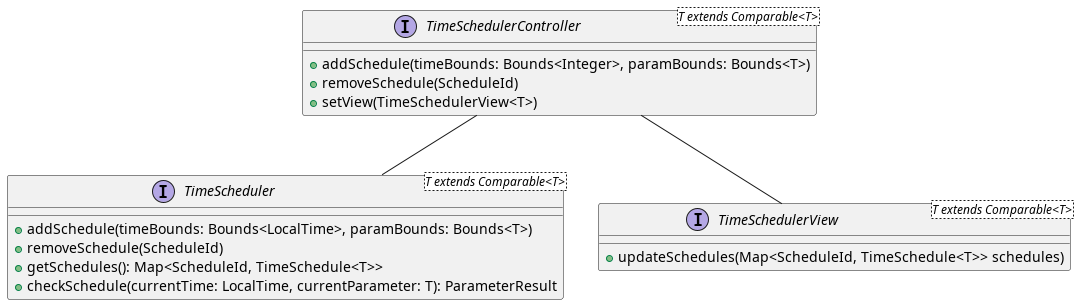
\includegraphics[width=\textwidth,height=\textheight,keepaspectratio]{magnani/uml/scheduler.png}
\caption{UML diagram of the scheduler overall structure}
\label{magnani:uml:scheduler}
\end{figure}

\subsubsection{Scheduler Model}

The scheduler model manages the storage of the schedules and the checking of the current parameter against the schedule.

\begin{figure}[H]
\centering{}
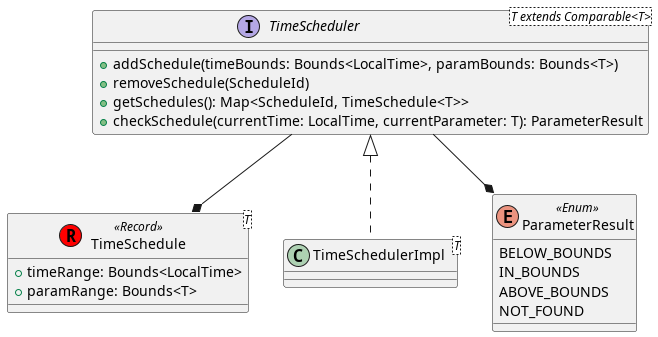
\includegraphics[width=\textwidth,height=\textheight,keepaspectratio]{magnani/uml/scheduler-model.png}
\caption{UML diagram of the scheduler model}
\label{magnani:uml:scheduler-model}
\end{figure}

\subsubsection{Scheduler Controller}

The scheduler controller handles the communication between the model and the view, and also implements the \texttt{DiscreteObject} interface
to periodically ask the model if the target parameter is met.
When the target parameter is not met, the scheduler will send a command to the domotic controller.

\begin{figure}[H]
\centering{}
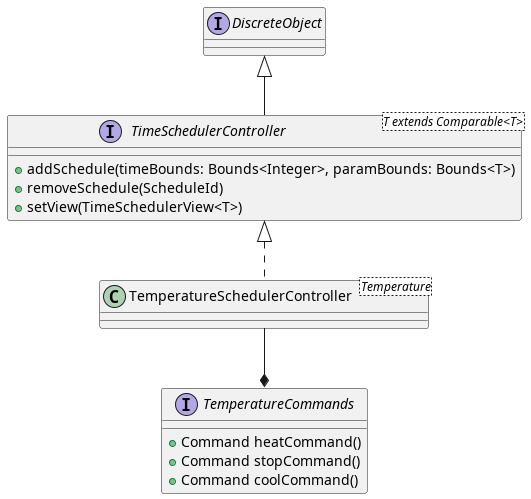
\includegraphics[width=\textwidth,height=\textheight,keepaspectratio]{magnani/uml/scheduler-controller.png}
\caption{UML diagram of the scheduler controller}
\label{magnani:uml:scheduler-controller}
\end{figure}

A \texttt{TemperatureCommands} interface has been created, following the \texttt{Strategy} pattern, to
specifically deal with the control of the temperature. \newline
Three separate commands are expected: heating, cooling, and stopping when the parameters are met.
In the proposed implementation, the heaters and air conditioners are instructed to set their state
to the minimum or maximum possible intensity, but for example, another implementation could
take into account the difference between the current temperature and the desired temperature,
and regulate the intensity proportionally.

A \texttt{Template} pattern has been used in \texttt{TemperatureCommand} to create this implementation,
with an abstract method \texttt{Function} to reuse the same code for both heating and cooling.
The template method is \texttt{setState}, as shown in figure \Cref{magnani:uml:temperaturecommand}.
This method is then used for both the heating and cooling functions.

\begin{figure}[H]
\centering{}
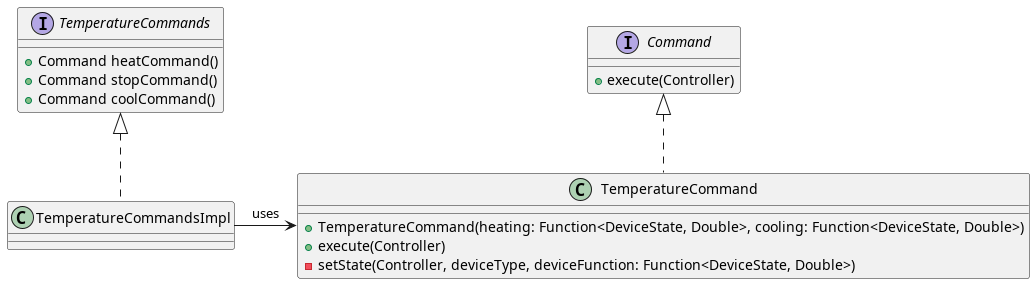
\includegraphics[width=\textwidth,height=\textheight,keepaspectratio]{magnani/uml/temperaturecommand.png}
\caption{UML diagram of the implementation of TemperatureCommands with the use of a template method in TemperatureCommand}
\label{magnani:uml:temperaturecommand}
\end{figure}

\subsubsection{Scheduler View}

The scheduler view has two tasks: allow the user to add/remove schedules, by calling the controller methods,
and displaying the current schedules, when updated from the controller.

\begin{figure}[H]
\centering{}
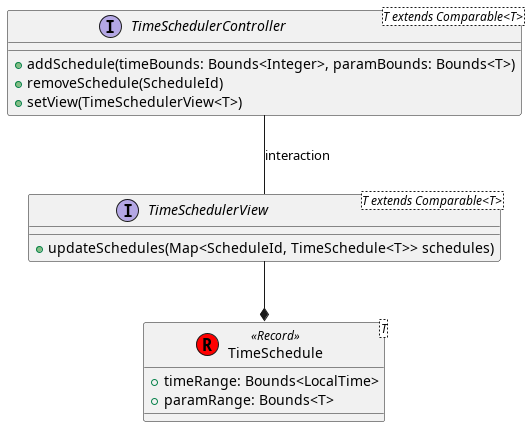
\includegraphics[width=\textwidth,height=\textheight,keepaspectratio]{magnani/uml/scheduler-view.png}
\caption{UML diagram of the scheduler view}
\label{magnani:uml:scheduler-view}
\end{figure}
